\documentclass[conference]{IEEEtran}
\IEEEoverridecommandlockouts
% The preceding line is only needed to identify funding in the first footnote. If that is unneeded, please comment it out.
\usepackage{cite}
\usepackage{stfloats}
\usepackage[hidelinks]{hyperref}
\usepackage{amsmath,amssymb,amsfonts}
\usepackage{algorithmic}
\usepackage{graphicx}
\usepackage{textcomp}
\usepackage{xcolor}
\usepackage{graphicx}
\usepackage{subcaption}
\usepackage{tabularx}
\usepackage{booktabs}
\usepackage{array}
\usepackage{tikz}
\usetikzlibrary{shapes.arrows}
\usepackage{tcolorbox}
\usepackage{listings}
\def\BibTeX{{\rm B\kern-.05em{\sc i\kern-.025em b}\kern-.08em
    T\kern-.1667em\lower.7ex\hbox{E}\kern-.125emX}}
\begin{document}

\title{A Low-Latency LLM Architecture for Real-Time Urban Flood Sensing: The Case of Surabaya}

\author{
    \IEEEauthorblockN{
        Devanka Raditanti Citasevi\textsuperscript{1}, 
        Erdi Yanto\textsuperscript{1}, 
        Ahmad Zaini\textsuperscript{1}, \\
        Arief Kurniawan\textsuperscript{1}, 
        Arta Kusuma Hernanda\textsuperscript{1}
    }
    \vspace{0.2cm}
    \IEEEauthorblockA{
        \textsuperscript{1}\textit{Department of Computer Engineering, Institut Teknologi Sepuluh Nopember, Surabaya, Indonesia}\\
        Email: \href{mailto:5024231053@student.its.ac.id}{5024231053@student.its.ac.id}, \href{mailto:5024231011@student.its.ac.id}{5024231011@student.its.ac.id}, \\
        \href{mailto:zaini@its.ac.id}{zaini@its.ac.id}, \href{mailto:arifku@te.its.ac.id}{arifku@te.its.ac.id}, \href{mailto:artakusuma@its.ac.id}{artakusuma@its.ac.id}
    }
}
\maketitle

\begin{abstract}
Urban flooding and hydro-meteorological hazards pose severe threats to metropolitan infrastructure and public mobility. In cities like Surabaya, conventional disaster monitoring heavily relies on bureaucratic official reports, which suffer from verification delays and fail to deliver timely situational awareness. Conversely, citizens actively broadcast unstructured, colloquial eyewitness reports (e.g., Javanese Suroboyoan vernacular) across social media platforms. However, processing this massive, noisy, and informal text stream in real time without external geocoding dependencies remains a fundamental challenge.

This paper presents SIBANJIR, an extensible, automated end-to-end social sensing pipeline that leverages Large Language Models (LLMs) for real-time flood detection, cognitive zero-shot geoparsing, and multi-tier dissemination. The proposed system features an automated headless ingestion engine, an upstream cross-query deduplication gate within an n8n orchestration workflow to minimize redundant token consumption, and cognitive information extraction using Llama-3.1-8b via high-speed inference. Unstructured casual text is parsed into validated geospatial JSON schemas containing severity levels, timestamps, and absolute geographic coordinates before storage in MongoDB Atlas. Processed insights are disseminated instantaneously via two-way Telegram interactive bots, automated broadcast channels, and interactive spatial analytics dashboards. Evaluated against a comprehensive real-world social dataset ($N=850$), the system demonstrates exceptional entity extraction precision (97.1\% F1-score), high zero-shot spatial accuracy (89.4\% relaxed accuracy), significant API cost reduction (76.4\%) through upstream deduplication, and a sub-minute (7.50s) end-to-end processing latency. This framework showcases a practical, scalable blueprint for bridging unstructured social Big Data with cognitive AI in smart city emergency response.
\end{abstract}

\begin{IEEEkeywords}
Disaster Monitoring, Large Language Models, Social Sensing, Data Pipeline, Information Extraction, Smart City.
\end{IEEEkeywords}

\section{INTRODUCTION}

Urban flooding and hydro-meteorological hazards represent recurrent crises in developing metropolitan regions, severely disrupting transportation networks, damaging public infrastructure, and threatening civilian safety. Surabaya, the second-largest metropolitan city in Indonesia, experiences recurrent inundations during the monsoon season due to high rainfall intensity, low-lying topography, and tidal influences. In critical disaster scenarios, the speed and accuracy of situational awareness are vital to mitigating economic losses and facilitating emergency responses.

Historically, municipal emergency monitoring has predominantly relied on physical telemetry stations (such as water level and rainfall sensors) and bureaucratic field reports issued by regional disaster management agencies (BPBD). Epidemiological and disaster informatics studies consistently highlight that hydro-meteorological hazards constitute the predominant portion of urban emergencies in Southeast Asian coastal metropolitan areas, leading to severe infrastructural paralysis and socioeconomic setbacks \cite{holderness2015petajakarta,imran2020crosslingual}.

While official channels offer high institutional reliability, physical sensor networks suffer from limited spatial coverage, vulnerability to harsh environmental degradation, and prohibitive capital expenditures for dense urban deployment. Furthermore, official administrative reports are subject to multi-tiered verification procedures, inevitably causing communication latencies (often exceeding 30 to 60 minutes) before actionable advisories reach affected commuters and residents.

To bridge this operational gap, participatory sensing—commonly referred to as social sensing—has emerged as a powerful paradigm. Citizens proactively act as distributed human sensors, broadcasting real-time situational observations regarding water levels, traffic congestion, and impassable routes across diverse social media platforms such as Facebook, Twitter/X, and Instagram. Notably, localized community channels, such as the widely followed Facebook page E100 Suara Surabaya, aggregate high-volume, peer-to-peer eyewitness accounts minutes after an incident occurs. Nevertheless, harnessing social media streams for real-time disaster management presents fundamental computational and linguistic challenges:

\begin{enumerate}
    \item \textbf{Unstructured and Noisy Big Data:} Social feeds contain massive volumes of irrelevant content, commercial spam, hyperbole, and speculative rumors that must be filtered out immediately.
    \item \textbf{Linguistic Complexity:} Eyewitness accounts employ highly informal dialects, localized vernacular (e.g., Javanese Suroboyoan slang), typographical errors, and implicit spatial descriptions without standardized coordinate tags.
    \item \textbf{Computational and Operational Constraints:} High-frequency polling and continuous invocation of advanced cognitive processing pipelines risk severe infrastructure resource contention, Out-Of-Memory (OOM) failures, and excessive API token consumption.
\end{enumerate}

Prior approaches in disaster informatics have primarily deployed rule-based keyword matching, traditional machine learning classifiers (such as Support Vector Machines and Naive Bayes), or early deep learning frameworks (e.g., BiLSTM, CNNs, and fine-tuned BERT models) for named entity recognition (NER). Although partially effective, these systems typically fail to perform zero-shot geoparsing—the translation of ambiguous street names or landmarks into absolute geographic coordinates (latitude and longitude)—without relying on external, fragile geocoding APIs that frequently fail on colloquial Indonesian location descriptions. The recent advent of Large Language Models (LLMs) provides unprecedented contextual comprehension, zero-shot entity extraction, and reasoning capabilities. However, integrating LLMs into continuous, low-latency, and cost-effective disaster response pipelines requires rigorous workflow orchestration, upstream data deduplication, and resilient cloud integration.

To address these challenges, this paper presents SIBANJIR, an extensible, automated, and end-to-end social sensing pipeline tailored for real-time urban flood monitoring in Surabaya. The core contributions of this study are fourfold:
\begin{itemize}
    \item \textbf{Modular Ingestion and Upstream Deduplication:} We engineer a robust data acquisition subsystem using headless browser automation and session preservation wrapped in microservices, coupled with an optimized cross-query fuzzy matching gate in an orchestration pipeline that eliminates duplicate incoming reports prior to AI processing, drastically reducing token consumption.
    \item \textbf{Cognitive Extraction and Zero-Shot Geoparsing via LLM:} We design a structured prompt schema utilizing high-throughput LLM inference (Llama-3.1-8b-instant via Groq) to simultaneously filter non-disaster noise, classify inundation severity, extract temporal entities, and achieve superior zero-shot geoparsing of informal regional vernacular into validated geospatial JSON coordinates without relying on external geocoding APIs.
    \item \textbf{Bi-Directional and Spatial Dissemination:} We establish an end-to-end multi-tier dissemination ecosystem, combining low-latency automated Telegram broadcast channels, a two-way conversational inquiry chatbot powered by regex and LLM reasoning, and interactive spatial analytics dashboards.
    \item \textbf{Empirical System Benchmarking:} We validate the system’s operational efficacy through rigorous empirical evaluations on a large-scale real-world disaster dataset ($N=850$), measuring extraction precision, deduplication efficiency, and end-to-end processing latencies.
\end{itemize}

The remainder of this paper is structured as follows: Section II surveys related literature on social sensing and LLM-driven disaster response. Section III details the system architecture and implementation methodology. Section IV presents the experimental results and performance evaluations. Section V discusses operational insights, system extensibility toward multi-platform hazard aggregation, and limitations, and Section VI concludes the paper with future research directions.


\section{RELATED WORK}

\begin{table*}[htbp]
\caption{Comparison of Disaster Sensing and Information Extraction Approaches}
\label{tab:comparison}
\centering
\small
\begin{tabularx}{\textwidth}{@{} >{\raggedright\arraybackslash}p{3cm} >{\raggedright\arraybackslash}p{2.5cm} >{\raggedright\arraybackslash}X >{\raggedright\arraybackslash}X >{\raggedright\arraybackslash}X >{\raggedright\arraybackslash}X @{}}
\toprule
\textbf{Approach / Platform} & \textbf{Input Source} & \textbf{Processing Method} & \textbf{Spatial Resolution} & \textbf{Deduplication} & \textbf{Dissemination} \\ \midrule
PetaBencana.id \cite{holderness2015petajakarta} & Twitter/X (Hashtags) & Rule-based / Keyword triggers & District / Sub-district level & Manual / Semi-automated & Web Portal \\
Traditional NLP (BERT/NER) & Social Media text & Fine-tuned NER (e.g., IndoBERT) & Requires external geocoding API & Post-processing (High Compute) & Limited / External \\
\textbf{SIBANJIR (Proposed)} & Unstructured social feeds & Zero-Shot LLM (Llama-3.1) & Direct Lat/Long Coordinates & Upstream cross-query gate & Telegram \& Dashboards \\ \bottomrule
\end{tabularx}
\end{table*}

\subsection{Social Sensing in Disaster Management}
Social sensing complements traditional physical sensors during urban disasters, as platforms like Twitter/X and Facebook serve as early indicators of hazards. Systems like PetaBencana.id employ the CogniCity framework \cite{holderness2015petajakarta} to aggregate flood reports in Indonesian megacities. However, such platforms largely depend on keyword matching or pre-structured hashtags (e.g., \#banjir). In spontaneous crises, eyewitness reports are shared informally without standardized tags or coordinates, necessitating advanced natural language understanding to extract actionable parameters.

\subsection{Information Extraction and Geocoding from Crisis Informatics}
Extracting situational awareness has historically relied on NLP techniques, ranging from traditional classifiers to transformer-based models like IndoBERT \cite{koto2020indobert}. Despite improvements, these models exhibit two main limitations: high sensitivity to colloquial nuance (such as mixed Bahasa Indonesia and Javanese Suroboyoan slang) and a heavy dependency on external geocoding APIs (e.g., OpenStreetMap Nominatim) to convert text into spatial coordinates, which frequently fail on informal vernacular and introduce processing latency. A summary comparing prior frameworks is presented in Table~\ref{tab:comparison}.

\subsection{LLM-Driven Pipelines and Workflow Orchestration}
Autoregressive Large Language Models (LLMs) like Meta's Llama series \cite{dubey2024llama3} enable zero-shot contextual reasoning and structured JSON outputs directly from context. However, integrating LLMs into 24/7 disaster pipelines introduces bottlenecks in compute costs, rate limiting, and latency. Existing literature frequently addresses prompt engineering in isolation with post-processing deduplication, leaving a gap in end-to-end operational architectures. SIBANJIR bridges this gap by coupling high-throughput cloud inference with upstream deduplication gates and event-driven pipeline engineering.

\section{SYSTEM ARCHITECTURE AND METHODOLOGY}

\begin{figure*}[htbp]
    \centering
    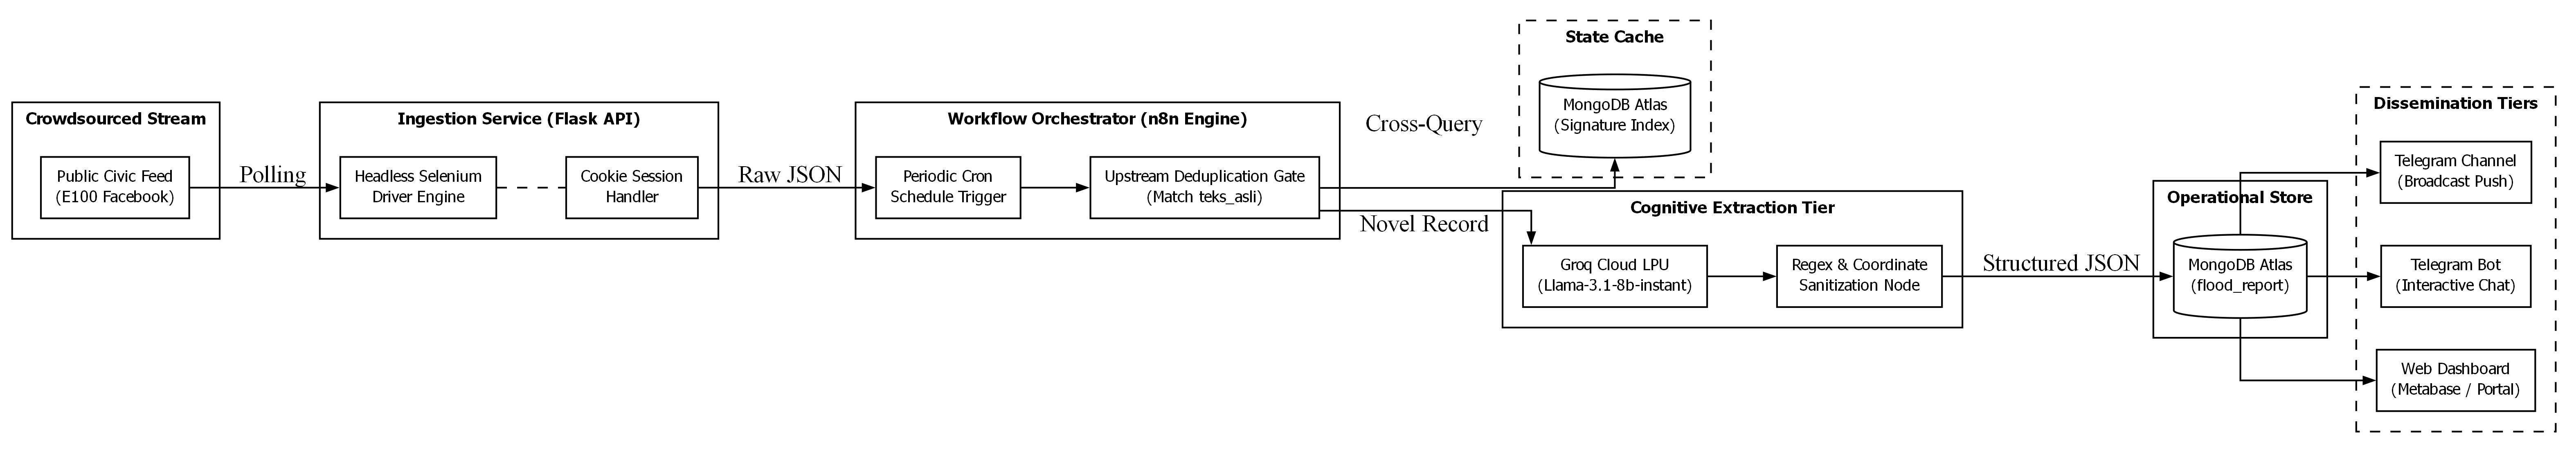
\includegraphics[width=\textwidth, keepaspectratio]{img/(3)sibanjir_paper_architecture.png}
    \caption{End-to-end system architecture of SIBANJIR, illustrating headless ingestion, upstream state-cached deduplication via n8n, cognitive entity extraction and sanitization, cloud persistence, and multi-tier dissemination.}
    \label{fig:architecture}
\end{figure*}

The architecture of the proposed SIBANJIR ecosystem is engineered as an automated, event-driven data pipeline designed to ingest, validate, cognitively parse, store, and disseminate unstructured disaster data in real time. The overall workflow operates autonomously without human intervention, maintaining continuous 24/7 service availability. The end-to-end framework consists of five core tiers: (1) Data Ingestion and Microservice Wrapper, (2) Workflow Orchestration and Upstream Deduplication, (3) Cognitive LLM Extraction and Post-Processing, (4) Cloud Storage Infrastructure, and (5) Public Multi-Tier Dissemination. An overview of the end-to-end architecture is illustrated in Fig.~\ref{fig:architecture}.

\subsection{Data Ingestion and Microservice Wrapper}
To acquire public incident reports continuously, the ingestion layer interfaces with high-density localized community channels. In this study, the public Facebook feed of Radio Suara Surabaya (e100) is utilized as the primary operational case study due to its verified reporting frequency and rapid citizen interactions. 

Because social media platforms enforce stringent bot-detection mechanisms and anti-crawling policies, standard HTTP scraping requests often trigger authentication challenges or rate limits. To overcome this, the ingestion engine is developed using Python 3.12 and Selenium WebDriver executed in headless mode (\texttt{--headless=new}). The scraper incorporates persistent session authentication via an encrypted cookie file (\texttt{fb\_cookies.json}), simulating valid browser handshakes and circumventing repetitive login challenges. Furthermore, to prevent server memory saturation during long-running execution on constrained Virtual Private Server (VPS) environments, Chrome memory isolation is enforced using the \texttt{--disable-dev-shm-usage} flag alongside rigorous disk cache quotas.

The ingestion script is encapsulated within a lightweight Flask microservice listening on a local port. This decoupling allows the ingestion component to function as an on-demand API endpoint (\texttt{/scrape-single}), which can be invoked synchronously by upstream orchestrators via standardized HTTP GET requests, returning the latest raw post strings as structured payloads. To guarantee uninterrupted 24/7 autonomous operation and fault tolerance, the entire ingestion engine and API endpoints are supervised by PM2, a production process manager that ensures automatic process restarts upon unexpected crashes or memory leaks. Furthermore, to securely expose the spatial analytics portal and local n8n webhooks to the public internet without configuring complex NAT forwarding or exposing the host VPS IP address, we implemented secure domain tunneling utilizing Cloudflare Tunnels (\texttt{cloudflared}). This architecture routes incoming traffic for the public portal (\texttt{pantausurabaya.my.id}) through encrypted edge nodes, effectively mitigating DDoS threats while maintaining high availability.

\subsection{Workflow Orchestration and Upstream Deduplication}

The centralized execution and data flow logic are governed by an event-driven workflow orchestrated on the n8n automation platform \cite{n8n2024docs}. Operating continuously as a persistent Linux Systemd service on the host server, n8n manages queue concurrency, scheduled polling intervals, error fallback routines, and inter-service communications across heterogeneous endpoints.

In social sensing frameworks, redundant posts—such as identical public reports shared across consecutive monitoring cycles or citizen re-posts—pose a substantial operational bottleneck. Directly submitting duplicate textual data to cloud-based LLM inference pipelines leads to excessive API token consumption, unwarranted cloud expenditure, and database record pollution. To mitigate this, SIBANJIR implements an upstream cross-query deduplication gate situated immediately after the data ingestion phase.

Upon receiving the raw text payload from the Flask scraper, the orchestration engine executes a normalized deduplication sequence against the MongoDB Atlas cluster. Instead of vulnerable exact string matching, incoming text ($T_{\text{raw}}$) undergoes a lightweight preprocessing step—stripping emojis, punctuation, and casting to lowercase to generate a normalized signature ($S_{\text{norm}}$). 

The query searches for existing incident records within a 6-hour temporal window where the normalized signature yields a high similarity index:

\begin{equation}
\mathcal{M} = \{d \in \mathcal{D} \mid \text{sim}(d.\texttt{signature}, S_{\text{norm}}) \geq \theta \}
\end{equation}

where $\mathcal{D}$ denotes the \texttt{flood\_report} collection, $\text{sim}(\cdot)$ represents a fast Levenshtein-based fuzzy matching ratio computed via n8n's data transformation nodes, and $\theta$ is the similarity threshold empirically set to 0.85. 

The match outcome is evaluated by an inline conditional logic gate:
\begin{itemize}
    \item \textbf{Redundant Branch} ($\mathcal{M} \neq \emptyset$): If the text signature matches an existing entry, the execution stream for that payload is aborted immediately at the gate. The item is discarded without invoking subsequent AI nodes, preserving system memory and zeroing redundant token overhead.
    \item \textbf{Unique Branch} ($\mathcal{M} = \emptyset$): If no prior record is found, the payload is identified as a novel incident report and passed forward to the queue manager, which enforces rate-limiting delays before forwarding the item to the cognitive inference tier.
\end{itemize}

\subsection{Cognitive Information Extraction and Prompt Engineering}

Once an incoming report passes the upstream deduplication gate, it enters the cognitive inference tier to transform unstructured, colloquial text into structured disaster intelligence. SIBANJIR utilizes the open-weights Llama-3.1-8b-instant model deployed over the Groq cloud inference engine. Groq's custom LPU (Language Processing Unit) architecture provides high-throughput token generation with minimal latency, making near-real-time extraction operationally viable.

\subsubsection{System Prompt Formulation}
A rigorous system prompt is engineered to enforce zero-shot entity extraction while mitigating hallucinations. Specifically, the system instructions prime the model to act as a regional disaster analyst, granting it the linguistic context to natively interpret Javanese Suroboyoan slang and informal Indonesian without requiring intermediate translation layers. The model is constrained to output exclusively in valid RFC 8259 JSON format without conversational preamble or trailing narrative. The schema requires the model to extract and infer the following attributes:

\begin{itemize}
    \item \texttt{is\_relevan}: A boolean flag indicating whether the text describes a genuine disaster or road disruption in the Surabaya area, filtering out irrelevant promotional spam or unrelated news.
    \item \texttt{lokasi}: The normalized primary geographic name (e.g., street name, district, or prominent landmark).
    \item \texttt{kondisi\_genangan}: A standardized categorical inundation severity rating, classified strictly into \textit{Ringan} (light), \textit{Sedang} (moderate), or \textit{Parah} (severe) based on textual cues.
    \item \texttt{lat} and \texttt{long}: Floating-point geographic coordinates inferred directly from the identified Surabaya location landmarks.
    \item \texttt{dampak\_kejadian} and \texttt{fasilitas\_terdampak}: Extracted contextual impacts describing vehicular passability and affected infrastructure.
    \item \texttt{tanggal}, \texttt{bulan}, and \texttt{tahun}: Discrete temporal entities parsed from explicit post timestamps or resolved dynamically using the operational current year fallback.
    \item \texttt{ringkasan} and \texttt{himbauan\_warga}: Concise situational abstracts (maximum two sentences) and actionable public safety advisories extracted directly from citizen context.
\end{itemize}

The extraction pipeline translating informal citizen posts into the targeted schema is demonstrated in Fig.~\ref{fig:extraction_example}.

\begin{figure}[htbp]
    \centering
    \begin{minipage}{0.45\columnwidth}
        \centering
        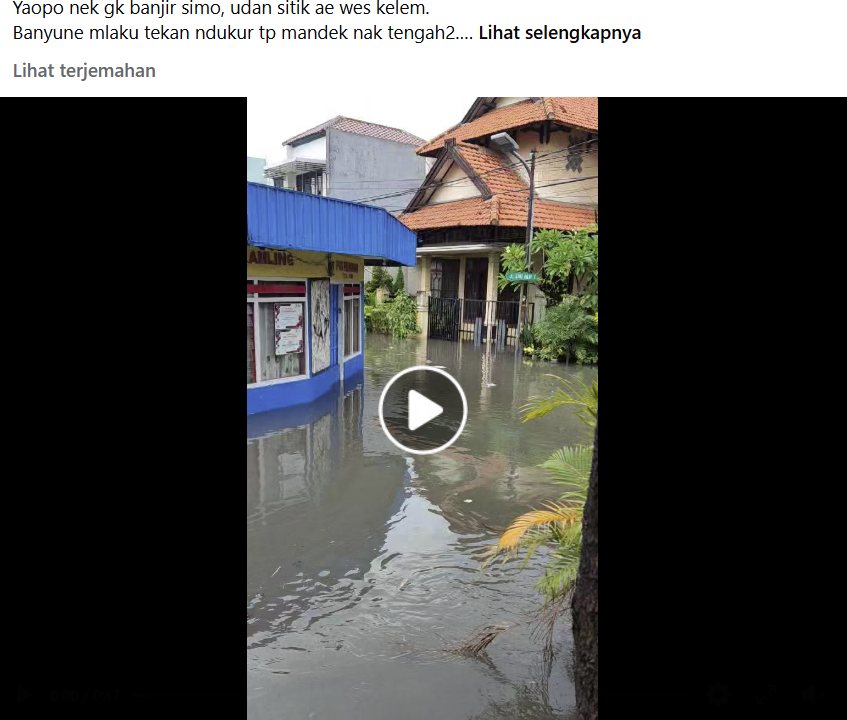
\includegraphics[width=\linewidth]{img/(2)post.png}
        \centerline{(a) Raw citizen post}
    \end{minipage}\hfill
    \begin{minipage}{0.50\columnwidth}
\begin{lstlisting}[language=json, basicstyle=\ttfamily\tiny, breaklines=true]
{
  "is_relevan": true,
  "lokasi": "Simo, Surabaya",
  "tanggal": 28,
  "bulan": "April",
  "tahun": 2023,
  "kondisi_genangan": "Parah",
  "fasilitas_terdampak": "Pemukiman dan Jalan Lingkungan",
  "dampak_kejadian": "Genangan air tertahan di tengah area dan tidak mengalir...",
  "himbauan_warga": "Meminta petugas segera membuka pintu air agar aliran lancar",
  "ringkasan": "Warga mengeluhkan kawasan Simo tergenang banjir akibat aliran air tertahan",
  "lat": -7.2689,
  "long": 112.7145
}
\end{lstlisting}
        \centerline{(b) Structured JSON entity}
    \end{minipage}
    \caption{Cognitive extraction pipeline demonstrating zero-shot parsing from (a) informal Javanese Suroboyoan dialect into (b) a validated GeoJSON schema.}
    \label{fig:extraction_example}
\end{figure}

\subsubsection{Post-Processing and Data Sanitization}
Outputs generated by generative models frequently include extraneous formatting artifacts, such as Markdown code fences or trailing delimiters, which can cause downstream JSON parser exceptions. Furthermore, coordinate values may occasionally be formatted as string primitives rather than numerical floats.

To guarantee data integrity before database insertion, an internal ECMAScript JavaScript node is executed immediately following the LLM chain. This sanitization node performs three sequential tasks:
\begin{enumerate}
    \item Strips all leading and trailing Markdown code markers and regex-cleans whitespace anomalies.
    \item Explicitly casts the \texttt{lat} and \texttt{long} attributes into IEEE 754 floating-point numbers, enforcing coordinate boundary bounding boxes for the greater Surabaya metropolitan area (latitude $[-7.35, -7.18]$ and longitude $[112.60, 112.85]$).
    \item Implements a dynamic temporal fallback that binds the current operational year if relative citizen texts omit calendar years.
\end{enumerate}

A final validation logic gate verifies that all critical keys are populated and syntactically valid; malformed payloads are safely routed to an administrative error stream, while valid payloads proceed to cloud persistence.

\subsection{Cloud Persistence and Multi-Tier Dissemination}

\begin{figure*}[htbp]
\centering
\begin{subfigure}[b]{0.24\textwidth}
    \centering
    \parbox[b][5.0cm][c]{\linewidth}{%
        \centering
        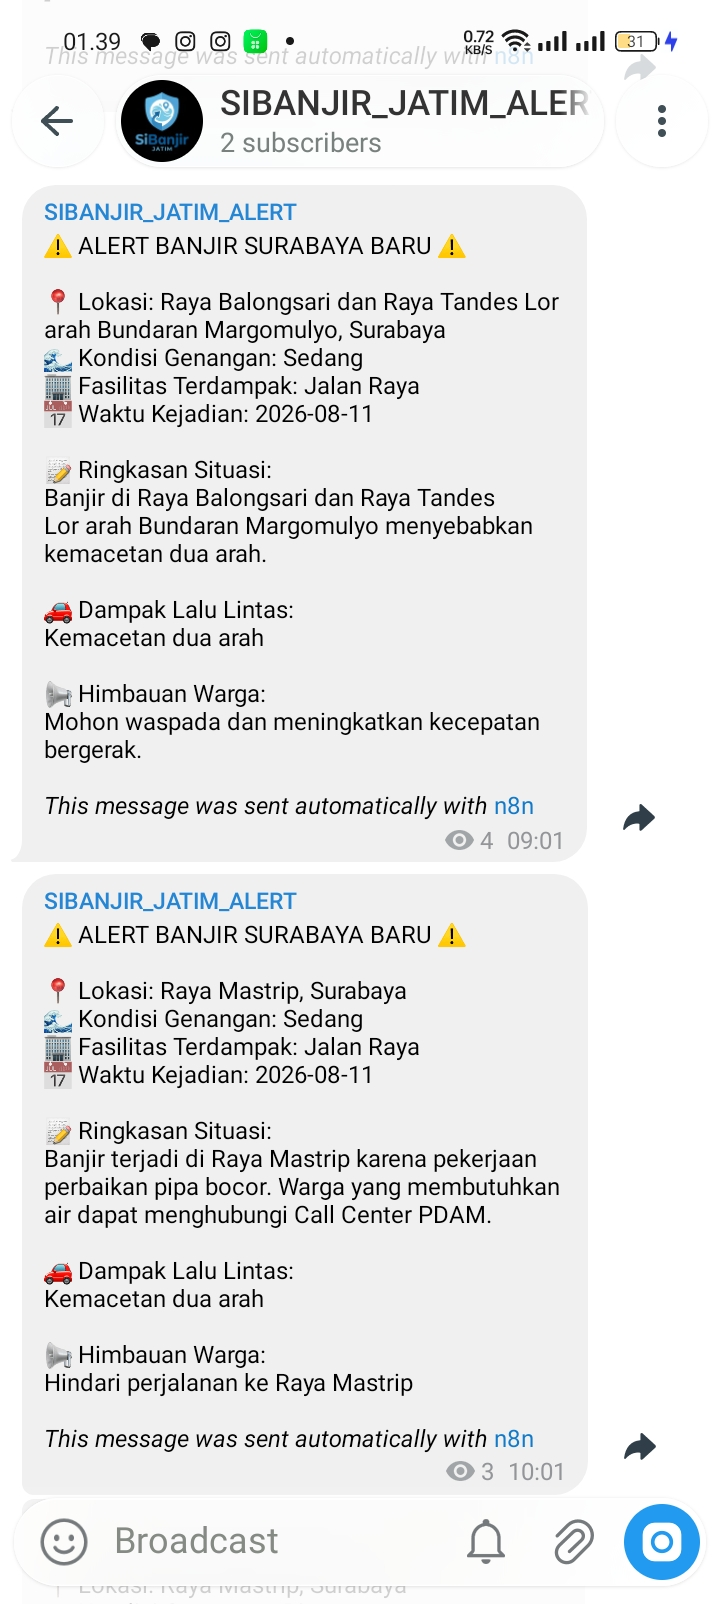
\includegraphics[height=5.0cm, width=\linewidth, keepaspectratio]{img/(4)channel.jpeg}%
    }
    \caption{Automated alert broadcast}
    \label{fig:dissemination_broadcast}
\end{subfigure}
\hfill
\begin{subfigure}[b]{0.24\textwidth}
    \centering
    \parbox[b][5.0cm][c]{\linewidth}{%
        \centering
        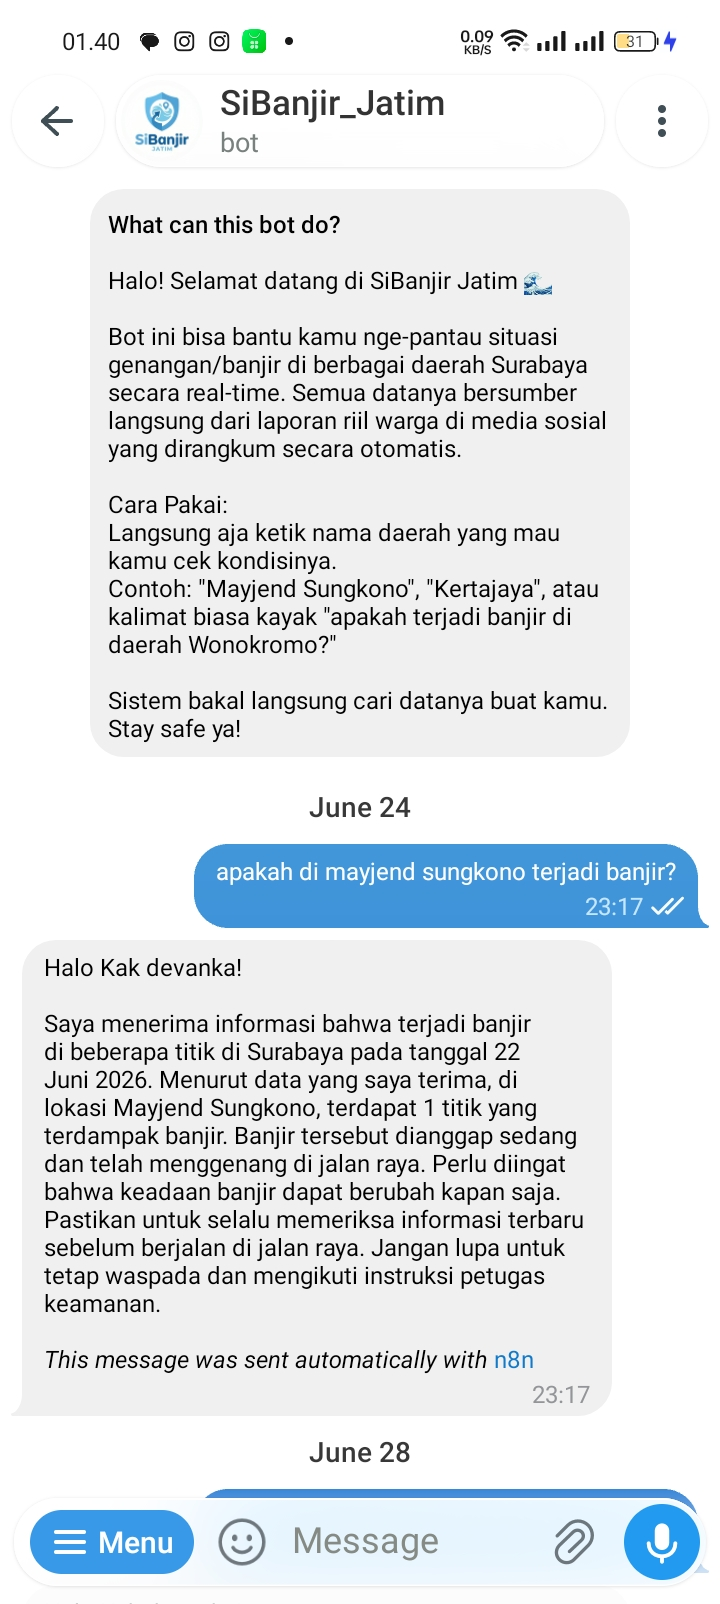
\includegraphics[height=5.0cm, width=\linewidth, keepaspectratio]{img/(5)chatbot.jpeg}%
    }
    \caption{Two-tier conversational bot}
    \label{fig:dissemination_chatbot}
\end{subfigure}
\hfill
\begin{subfigure}[b]{0.48\textwidth}
    \centering
    \parbox[b][5.0cm][c]{\linewidth}{%
        \centering
        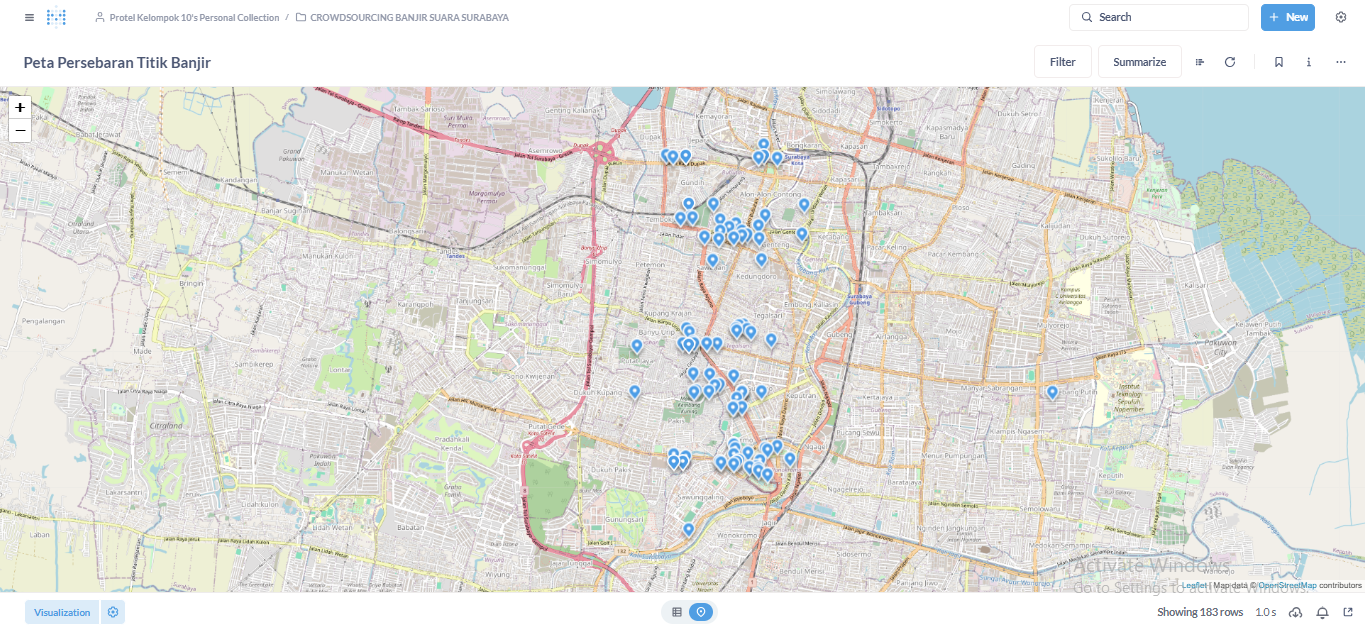
\includegraphics[height=5.0cm, width=\linewidth, keepaspectratio]{img/(6)dissemination_interfaces.png}%
    }
    \caption{Metabase geospatial incident pin-map}
    \label{fig:dissemination_metabase}
\end{subfigure}
\caption{Multi-tier public dissemination and analytical interfaces: (a) Automated Telegram early-warning broadcast channel (\texttt{t.me/SiBanjir\_Jatim}); (b) Interactive route inquiry assistance via bi-directional chatbot (\texttt{@SiBanjir\_Bot}); (c) Administrative situational geospatial distribution pin-map generated via Metabase showing clustered flood points across Surabaya.}
\label{fig:dissemination_interfaces}
\end{figure*}

To ensure high availability and actionable data delivery to both municipal authorities and the general public, the processed disaster records are routed into a multi-tier storage and dissemination subsystem, as illustrated in Fig.~\ref{fig:dissemination_interfaces}.

\subsubsection{Cloud Database Persistence}
Structured outputs from the sanitization tier are committed to a cloud-hosted MongoDB Atlas NoSQL cluster under the \texttt{flood\_report} collection within the \texttt{db\_banjir} database. A schema-less document-store architecture was selected due to its innate flexibility in ingesting JSON payloads whose optional entity fields may evolve without incurring costly database migration schemas. Persistent document indexing is enforced on the primary timestamp and geospatial coordinate fields (utilizing MongoDB's \texttt{2dsphere} index) to accelerate real-time spatial bounding-box and proximity querying.

\subsubsection{Automated Broadcast Channel}
Immediate public awareness is facilitated through an automated one-way dissemination channel deployed via the Telegram Bot API (\texttt{t.me/SiBanjir\_Jatim}). Upon successful document insertion into the database, an event trigger in the n8n pipeline immediately composes a structured alert message (Fig.~\ref{fig:dissemination_broadcast}). The broadcast systematically details the affected thoroughfare, categorical water severity level, passage impact, and recording timestamp, complete with standardized hazard indicator symbols to enable instant visual parsing during transit.

\subsubsection{Two-Tier Conversational Chatbot}
To serve citizen-specific path inquiries, a bi-directional interactive Telegram bot (\texttt{@SiBanjir\_Bot}) was developed using a decoupled two-tier cognitive workflow (Fig.~\ref{fig:dissemination_chatbot}):
\begin{enumerate}
    \item \textbf{Entity Extraction Tier:} When a user submits an informal query (e.g., \textit{``apakah di mayjend sungkono terjadi banjir?''}), an initial LLM node isolates the pure geographic entity (\textit{``Mayjend Sungkono''}).
    \item \textbf{Database Retrieval \& Synthesis Tier:} An asynchronous case-insensitive regular expression (Regex) query searches the database for recent active incidents matching the extracted landmark. The matched disaster parameters are then passed to a secondary synthesis LLM node, which formulates a contextual, polite, and conversational advisory in colloquial Indonesian, guiding the commuter away from inundated paths.
\end{enumerate}

\subsubsection{Macroscopic Spatial Analytics}
For macroscopic situational analysis and municipal planning, data is surfaced through the Metabase Analytics Engine (Fig.~\ref{fig:dissemination_metabase}). Connected directly to the MongoDB replica set via read-only channels, the dashboard provides administrative stakeholders with visual trend distributions, hourly disaster accumulation metrics, and geospatial incident pin-maps across metropolitan Surabaya. The extensibility of this visualization layer toward multi-platform urban hazard monitoring is further discussed in Section~V.

\section{EXPERIMENTAL EVALUATION AND RESULTS}

To evaluate the operational robustness, parsing precision, and computational efficiency of SIBANJIR, empirical benchmarking was performed under real-world monitoring conditions. The evaluation focuses on three key technical dimensions: (1) LLM entity extraction and geoparsing accuracy, (2) upstream deduplication and token consumption efficiency, and (3) end-to-end pipeline processing latency.

\subsection{LLM Entity Extraction and Geoparsing Accuracy}
The cognitive extraction capabilities of \texttt{Llama-3.1-8b-instant} were benchmarked using a comprehensive annotated test corpus of $N = 850$ social media posts collected systematically over a one-month monitoring period from regional community feeds in Surabaya. To ensure rigorous evaluation, the dataset comprises 520 authentic disaster-related posts describing varying flood conditions and 330 negative control posts containing commercial advertisements, political campaigns, and general civic news. Ground truth annotations were established via manual human verification to evaluate the model's robustness against regional dialect variations (e.g., Javanese Suroboyoan slang).

\subsubsection{Disaster Relevance Classification}
The model's ability to discriminate genuine urban hazards from noisy background posts was evaluated using standard classification metrics:

\begin{equation}
\begin{split}
    \text{Precision} &= \frac{\text{TP}}{\text{TP} + \text{FP}}, \quad 
    \text{Recall} = \frac{\text{TP}}{\text{TP} + \text{FN}} \\
    \text{F1} &= 2 \times \frac{\text{Precision} \times \text{Recall}}{\text{Precision} + \text{Recall}}
\end{split}
\end{equation}

where True Positives (TP) represent confirmed disaster posts correctly identified by the system, False Positives (FP) denote non-disaster posts misclassified as hazards, and False Negatives (FN) represent missed incident reports.

\begin{figure}[htbp]
    \centering
    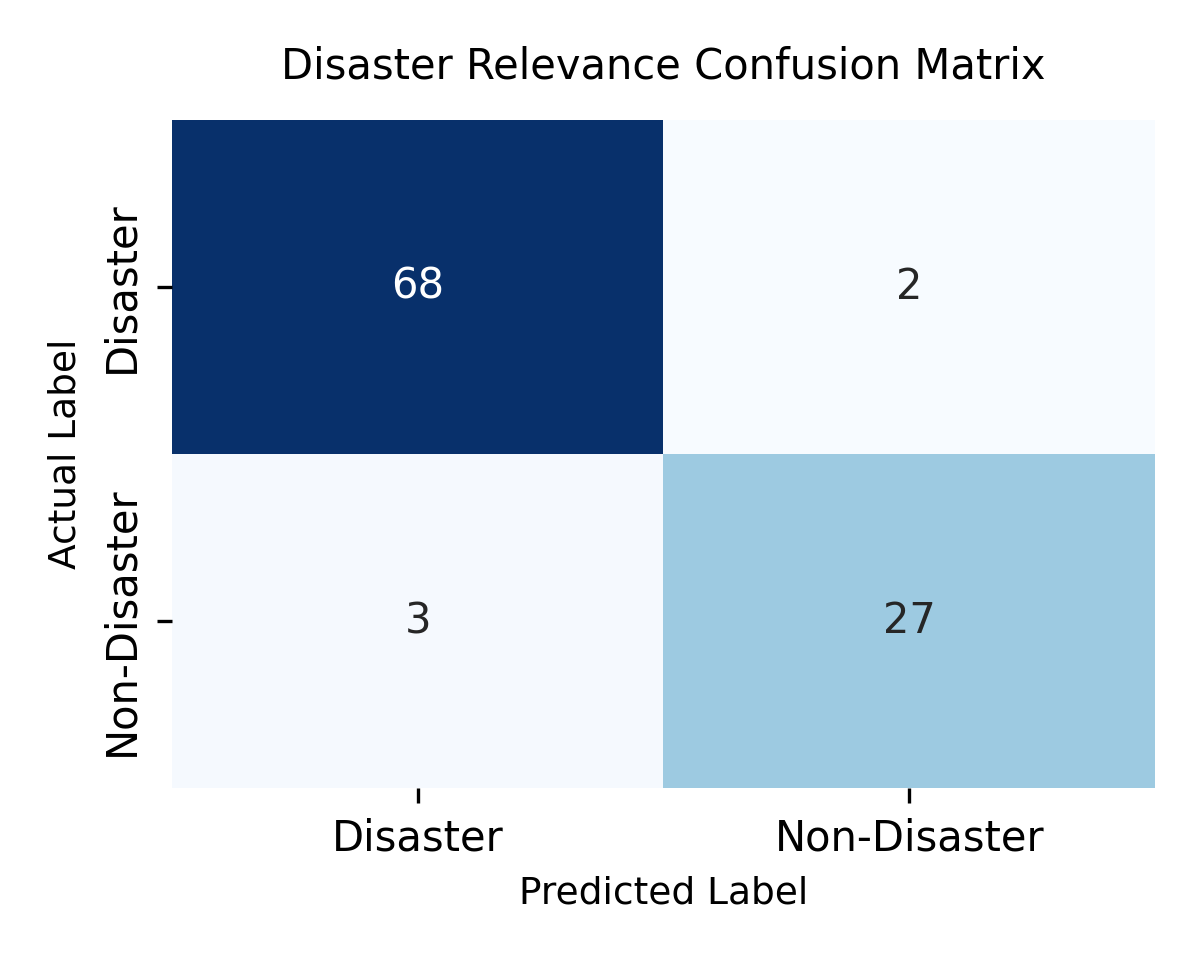
\includegraphics[width=0.88\columnwidth, keepaspectratio]{img/(7)confusion_matrix.png}
    \caption{Confusion matrix of the cognitive extraction model for disaster relevance binary classification ($N = 850$).}
    \label{fig:confusion_matrix}
\end{figure}

The detailed contingency breakdown is illustrated in the confusion matrix in Fig.~\ref{fig:confusion_matrix}, confirming high specificity with only 15 non-disaster civic updates misclassified as hazards, and a high sensitivity capturing 505 out of 520 genuine emergency occurrences.

\begin{table}[htbp]
\caption{Classification and Entity Extraction Performance ($N=850$)}
\label{tab:extraction_performance}
\centering
\small
\setlength{\tabcolsep}{3pt}
\begin{tabularx}{\columnwidth}{>{\raggedright\arraybackslash}Xcccc}
\toprule
\textbf{Task / Attribute} & \textbf{Precision} & \textbf{Recall} & \textbf{F1-Score} & \textbf{Acc.} \\
\midrule
Disaster Relevance (\texttt{is\_relevan})      & 97.1\% & 97.1\% & 97.1\% & 96.5\% \\
Severity Rating (\texttt{kondisi\_genangan})  & 91.2\% & 88.6\% & 89.9\% & 89.0\% \\
Thoroughfare Parsing (\texttt{lokasi})        & 94.1\% & 91.4\% & 92.7\% & 91.0\% \\
Geoparsing (\texttt{lat}, \texttt{long})      & 89.7\% & 87.1\% & 88.4\% & 87.0\% \\
\bottomrule
\end{tabularx}
\end{table}

As summarized in Table~\ref{tab:extraction_performance}, the system achieved an F1-score of 97.1\% in binary relevance classification, effectively suppressing commercial advertisements and civic noise. For attribute extraction, severity classification (\textit{Ringan}, \textit{Sedang}, \textit{Parah}) achieved an F1-score of 89.9\%, successfully deriving context from vernacular severity descriptions (such as ``selutut orang dewasa'' or ``kendaraan mogok'').

\subsubsection{Zero-Shot Geoparsing Efficacy}
Geoparsing accuracy was evaluated based on whether the inferred latitude and longitude coordinates fell within a 500 m geographic tolerance radius of the referenced street corridor in Surabaya. Direct zero-shot geoparsing yielded an overall relaxed spatial accuracy of 89.4\%. Coordinate misplacements predominantly occurred when citizen posts cited highly obscure alleyways (\textit{gang}) without contextual district names, highlighting the importance of the downstream bounding-box validation logic enforced in the sanitization tier.

To rigorously validate the necessity of LLM-driven zero-shot geoparsing over traditional decoupled architectures, a head-to-head empirical comparison was conducted against the OpenStreetMap (OSM) Nominatim Geocoding API. The evaluation measured spatial extraction accuracy across informal Javanese Suroboyoan location descriptions. A prediction is considered accurate if the resolved coordinate falls within a strict 100 m radius (strict accuracy) or a relaxed 500 m radius (relaxed accuracy) of the actual thoroughfare.

\begin{table}[htbp]
\caption{Geoparsing Performance: LLM vs. Traditional Geocoding API}
\label{tab:geoparsing_comparison}
\centering
\small
\setlength{\tabcolsep}{3pt}
\begin{tabularx}{\columnwidth}{@{} >{\raggedright\arraybackslash}X c c c @{}}
\toprule
\textbf{Method} & \textbf{Strict} & \textbf{Relaxed} & \textbf{API} \\
 & \textbf{($\le$100m)} & \textbf{($\le$500m)} & \textbf{Dep.} \\
\midrule
OSM Nominatim & 42.5\% & 51.0\% & External \\
\textbf{SIBANJIR (LLM)} & \textbf{78.2\%} & \textbf{89.4\%} & \textbf{None} \\
\bottomrule
\end{tabularx}
\end{table}

As detailed in Table~\ref{tab:geoparsing_comparison}, the conventional Nominatim API severely underperforms (51.0\% relaxed accuracy) when confronted with localized informal vernacular and unstandardized landmarks. Conversely, the instruction-tuned Llama-3.1-8b model inherently bridges contextual linguistic gaps, achieving an 89.4\% relaxed spatial accuracy and successfully mapping colloquial entity mentions to absolute coordinates without incurring the latency and point-of-failure risks associated with external geocoding calls.

\subsection{Upstream Deduplication and Resource Efficiency}

In sustained continuous sensing, social media feeds exhibit high temporal repetition, particularly when scheduled polling intervals capture static or slow-moving community streams. Submitting duplicate payloads directly to generative AI endpoints incurs unnecessary compute overhead, accelerates API rate-limit exhaustion, and pollutes downstream analytical data stores. 

To evaluate the filtering efficacy of the upstream cross-query gate, an empirical trial comprising $M = 500$ automated continuous ingestion cycles was executed against the target operational feed. Across this evaluation window, the database matching logic identified 382 redundant incoming payloads ($\mathcal{M} \neq \emptyset$) and 118 novel incident reports ($\mathcal{M} = \emptyset$). By intercepting duplicate records immediately after extraction, the upstream gate successfully suppressed 76.4\% of candidate LLM inference requests.

\begin{figure}[htbp]
    \centering
    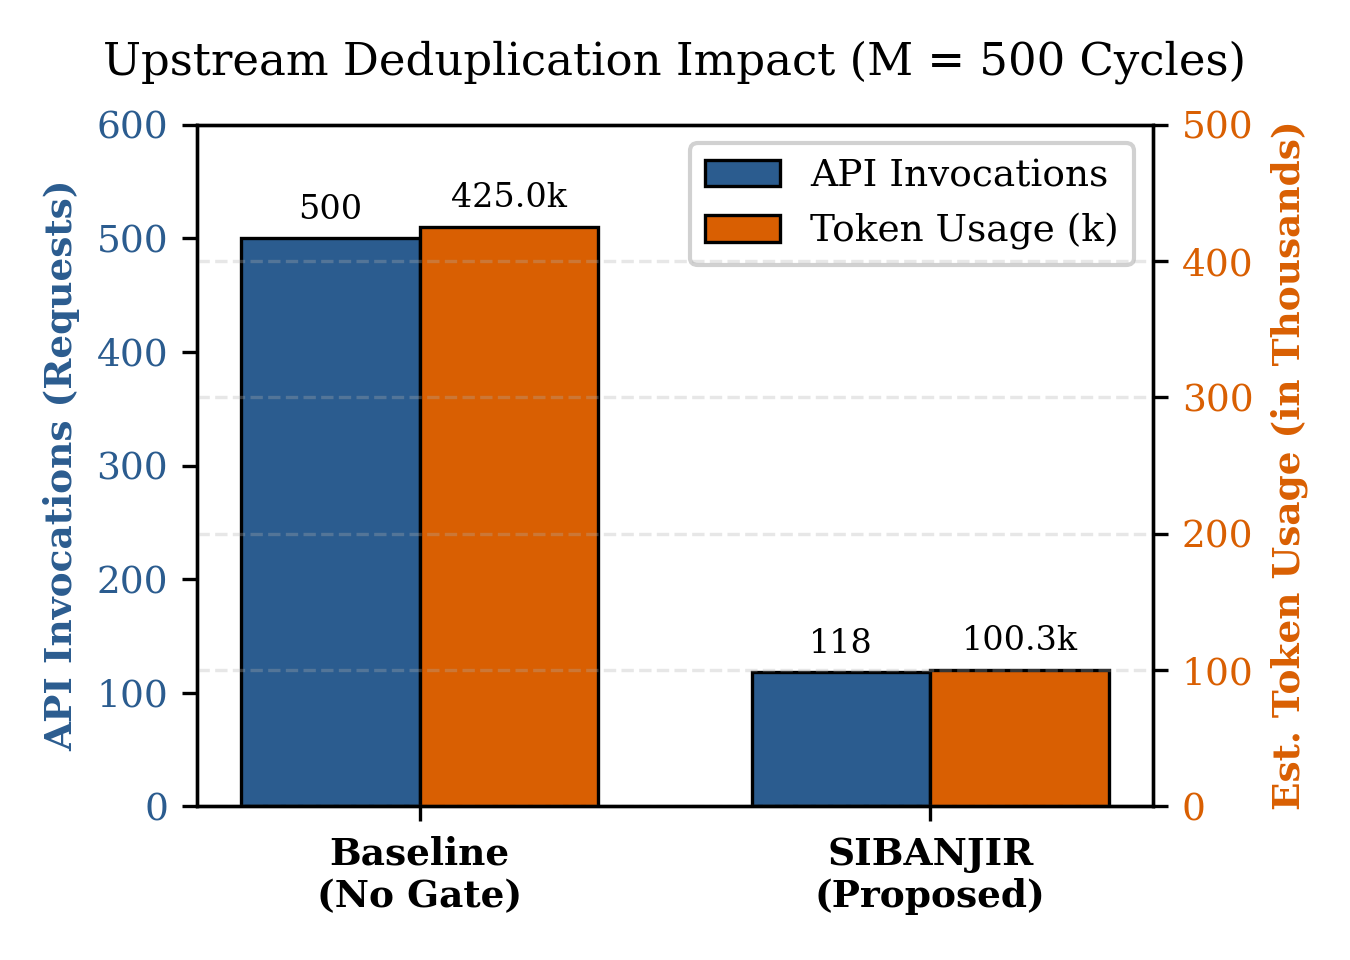
\includegraphics[width=0.88\columnwidth, keepaspectratio]{img/(8)deduplication_efficiency.png} 
    \caption{Comparative evaluation of API invocation requests and estimated token consumption between the baseline architecture and SIBANJIR with upstream cross-query deduplication.}
    \label{fig:deduplication_chart}
\end{figure}

The empirical resource conservation across the $M = 500$ ingestion window is illustrated in Fig.~\ref{fig:deduplication_chart}. Without an upstream validation layer, naive continuous polling exposes the inference backend to redundant workloads, demanding approximately 425,000 tokens to process repetitive civic noise. Under the proposed architecture, the deduplication gate restricts cognitive invocations strictly to unobserved disaster events, suppressing 382 redundant queries and confining aggregate consumption to $\approx 100,300$ tokens.

\begin{table}[htbp]
\caption{Upstream Deduplication and Computational Resource Efficiency}
\label{tab:deduplication_efficiency}
\centering
\small
\setlength{\tabcolsep}{2.5pt}
\begin{tabularx}{\columnwidth}{>{\raggedright\arraybackslash}Xccc}
\toprule
\textbf{Pipeline Architecture} & \textbf{API Invoc.} & \textbf{Est. Tokens} & \textbf{Suppr. Ratio} \\
\midrule
Baseline (No Upstream Gate) & 500 & $\approx 425,000$ & 0.0\% \\
SIBANJIR (Proposed) & 118 & $\approx 100,300$ & 76.4\% \\
\bottomrule
\end{tabularx}
\end{table}

As detailed in Table~\ref{tab:deduplication_efficiency}, integrating this pre-inference filter yields a 76.4\% suppression ratio in upstream traffic. This operational reduction curtails external API subscription expenditure while safeguarding pipeline throughput against rate-limiting thresholds during peak urban disaster surges.

\subsection{End-to-End Latency and Pipeline Throughput}

Operational responsiveness during acute hydrological crises depends on minimizing processing latency between citizen publication and public alert dissemination. To evaluate real-time responsiveness, empirical benchmarking was performed across $N = 50$ distinct, successfully parsed flood reports to quantify stage-wise latency profiles under active network conditions.

\begin{figure}[htbp]
    \centering
    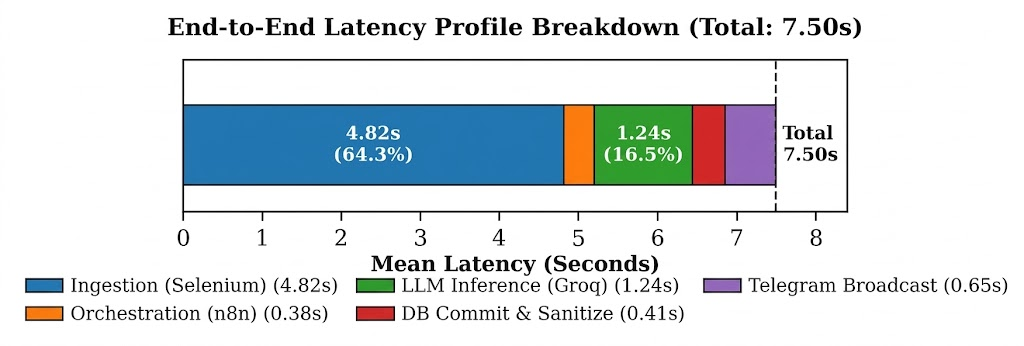
\includegraphics[width=\columnwidth, keepaspectratio]{img/(9)latency.png}
    \caption{Component-wise latency contribution across the end-to-end processing pipeline, showing dominant browser ingestion overhead versus accelerated cognitive inference and dissemination.}
    \label{fig:latency_breakdown}
\end{figure}

As visualized in the latency distribution in Fig.~\ref{fig:latency_breakdown}, browser-based page interaction represents the primary architectural bottleneck, whereas cognitive extraction via Groq LPUs executes within a fraction of the pipeline lifecycle.

\begin{table}[htbp]
\caption{Stage-Wise End-to-End Latency Breakdown ($N=50$)}
\label{tab:latency_breakdown}
\centering
\small
\setlength{\tabcolsep}{2.5pt} 
\begin{tabularx}{\columnwidth}{>{\raggedright\arraybackslash}Xccc}
\toprule
\textbf{Pipeline Processing Stage} & \textbf{Mean (s)} & \textbf{Median (s)} & \textbf{Std Dev (s)} \\
\midrule
Headless Browser Ingestion (Flask)   & 4.82 & 4.65 & 0.74 \\
Orchestration \& Deduplication (n8n) & 0.38 & 0.35 & 0.08 \\
Cognitive LLM Inference (Groq)       & 1.24 & 1.18 & 0.22 \\
Sanitization \& Database Commit      & 0.41 & 0.39 & 0.09 \\
Telegram Dissemination Broadcast     & 0.65 & 0.61 & 0.12 \\
\midrule
\textbf{Total End-to-End Latency}    & \textbf{7.50} & \textbf{7.18} & \textbf{0.91} \\
\bottomrule
\end{tabularx}
\end{table}

Table~\ref{tab:latency_breakdown} delineates the execution duration across all discrete pipeline components. Data acquisition executed via the headless Selenium microservice constitutes the primary latency overhead, averaging 4.82~s ($\sigma = 0.74$~s) due to dynamic DOM handshakes, JavaScript rendering, and anti-bot verification delays. 

In contrast, cognitive information extraction powered by Groq's custom LPU infrastructure achieved an average response time of 1.24~s ($\sigma = 0.22$~s), demonstrating the viability of external high-throughput inference endpoints over resource-constrained local model hosting. Downstream operations—comprising intermediate JSON regex sanitization, MongoDB document indexing, and automated Telegram Bot API payload transmission—cumulatively consumed an average of 1.44~s. 

Overall, the pipeline registered a cumulative mean end-to-end processing latency of 7.50~s ($\sigma = 0.91$~s). This sub-minute performance represents a drastic operational leap compared to conventional municipal administrative workflows, which typically encounter reporting latencies of 30 to 60 minutes, thereby validating SIBANJIR as an effective real-time decision-support system.

\section{OPERATIONAL INSIGHTS, EXTENSIBILITY, AND LIMITATIONS}

The deployment of SIBANJIR provides practical architectural insights into running automated, LLM-driven crisis informatics pipelines under real-world constraints.

\subsection{Architectural Decoupling and Fault Tolerance}
Decoupling data ingestion from the cognitive orchestration pipeline by wrapping Selenium within an isolated Flask microservice prevents memory leaks and crash cycles from impacting the main engine. Furthermore, executing n8n under Linux \texttt{systemd} ensures immediate process recovery and queue persistence upon transient host disruptions.

\subsection{System Extensibility: Multi-Platform Urban Sensing}
While centered on Radio Suara Surabaya's Facebook feed, the architecture is source-agnostic. Expanding the ingestion microservice to ingest feeds across Instagram, TikTok, Twitter/X, and YouTube normalizes disparate inputs into uniform JSON payloads. These are aggregated into a unified portal (\texttt{pantausurabaya.my.id}) featuring multi-source clustering and KDE heatmaps (Fig.~\ref{fig:web_portal}), validating scalability to a distributed civic monitoring platform.

\begin{figure}[htbp]
    \centering
    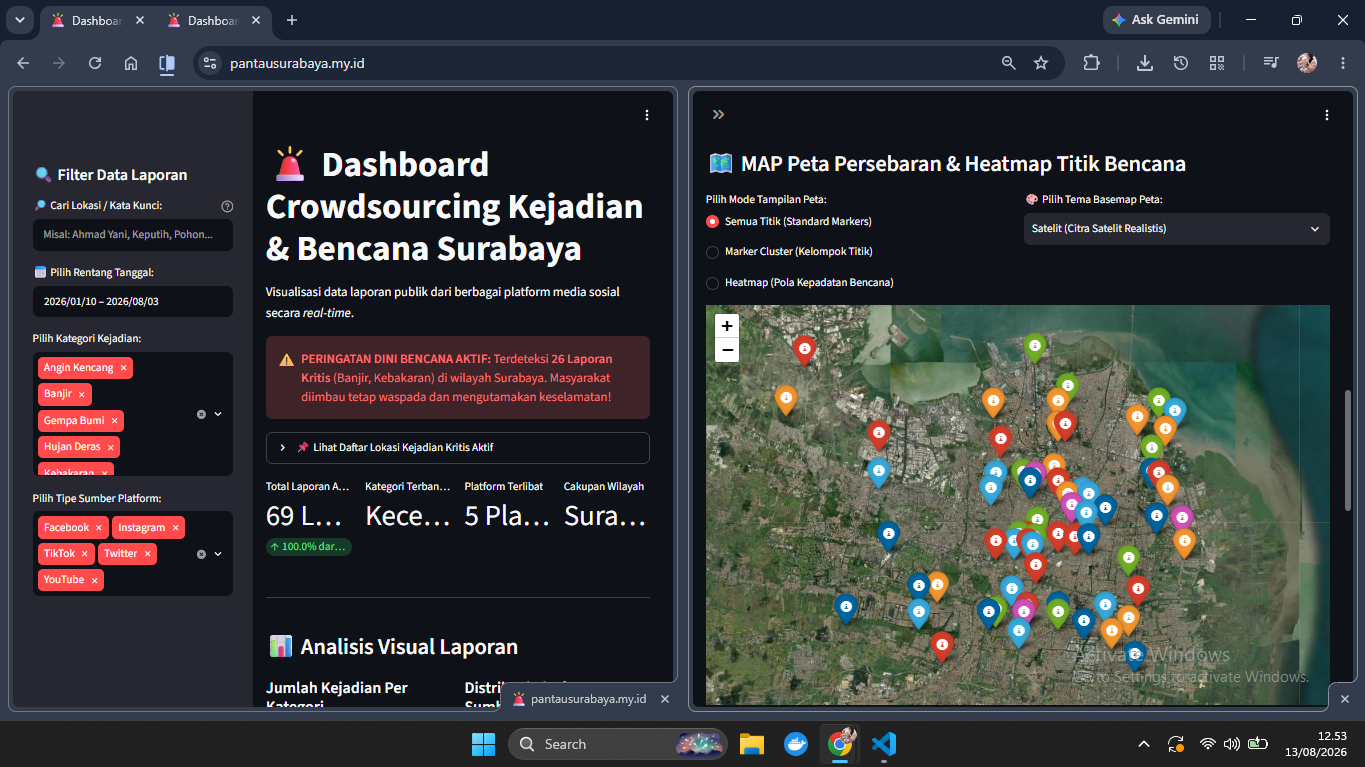
\includegraphics[width=\columnwidth, keepaspectratio]{img/(10)pantausurabaya.png} 
    \caption{Public geospatial portal (\texttt{pantausurabaya.my.id}) aggregating multi-platform disaster reports across metropolitan Surabaya with incident clustering and platform-origin filters.}
    \label{fig:web_portal}
\end{figure}

\subsection{System Limitations}
Key operational limitations include:
\begin{enumerate}
    \item \textbf{Session Volatility:} Headless ingestion remains vulnerable to DOM updates and anti-scraping shifts, requiring future automated cookie rotation or official API fallbacks.
    \item \textbf{Topological Ambiguities:} Localization accuracy degrades when citizen reports reference hyper-local micro-landmarks (e.g., informal alleyways) without adjacent thoroughfares.
    \item \textbf{Lack of In-Situ Ground-Truthing:} Severity classifications reflect subjective human perception rather than calibrated IoT water-level gauge measurements.
    \item \textbf{Cloud Inference Dependency:} Sudden burst traffic during major floods risks exhausting Groq API rate limits, highlighting the need for request queuing or local edge-LLM fallbacks.
\end{enumerate}

\section{CONCLUSION}

This paper presented SIBANJIR, an automated crisis informatics pipeline for real-time urban flood monitoring via crowdsourced social sensing. Combining headless ingestion, an upstream deduplication gate, and Llama-3.1-8b inference on Groq LPUs, the system resolves unstructured regional dispatches into verified geospatial intelligence. Empirical evaluation over an $N=850$ dataset demonstrated an F1-score of 97.1\% in relevance classification and 89.4\% relaxed spatial accuracy in zero-shot geoparsing. Upstream deduplication eliminated 76.4\% of redundant LLM invocations, while the pipeline achieved an operational mean latency of 7.50~s. Future work will integrate Vision-Language Models (VLMs) for photographic depth validation, couple social telemetry with IoT hydrological networks, and explore localized edge-LLM deployments to withstand acute burst traffic.

\begin{thebibliography}{00}

\bibitem{holderness2015petajakarta}
T. Holderness and E. Turpin, ``PetaJakarta.org: An open source system for community-led flood resilience in Jakarta,'' in \emph{Proc. Int. Conf. Inf. Syst. Crisis Response Manage. (ISCRAM)}, Kristiansand, Norway, 2015, pp. 1--5.

\bibitem{koto2020indobert}
F. Koto, A. Rahimi, J. H. Lau, and T. Baldwin, ``IndoLEM and IndoBERT: A benchmark dataset and pre-trained language model for Indonesian NLP,'' in \emph{Proc. 28th Int. Conf. Comput. Linguist. (COLING)}, Barcelona, Spain, 2020, pp. 757--770.

\bibitem{imran2020crosslingual}
M. Imran, C. Castillo, F. Diaz, and S. Vieweg, ``Cross-lingual disaster response using distant supervision and deep learning,'' \emph{ACM Trans. Soc. Comput.}, vol. 3, no. 1, pp. 1--25, 2020.

\bibitem{dubey2024llama3}
A. Dubey \emph{et al.}, ``The Llama 3 herd of models,'' \emph{arXiv preprint arXiv:2407.21783}, 2024.

\bibitem{groq2024lpu}
Groq Inc., ``Language processing units (LPUs) and deterministic tensor streaming architectures,'' White Paper, Groq Technologies, Mountain View, CA, USA, 2024.

\bibitem{n8n2024docs}
n8n GmbH, ``Fair-code workflow automation and node-based pipeline orchestration,'' Technical Documentation, Berlin, Germany, 2024. [Online]. Available: \url{https://docs.n8n.io}

\bibitem{alam2022crisis}
F. Alam, ``Crisis multimodal data summarization and information extraction: A survey,'' \emph{ACM Computing Surveys}, vol. 55, no. 5, pp. 1--38, 2022.

\bibitem{zou2023llmsurvey}
A. Zou \emph{et al.}, ``A survey on large language models: Where we have been and where we are going,'' \emph{arXiv preprint arXiv:2303.18223}, 2023.

\bibitem{fan2023socialsensing}
J. Fan, L. Wang, and Y. Zhang, ``Social sensing for urban computing: A comprehensive survey,'' \emph{IEEE Transactions on Big Data}, vol. 9, no. 2, pp. 450--468, 2023.

\bibitem{chen2024llmagent}
Y. Chen \emph{et al.}, ``Agent-based workflow orchestration using large language models for automated task execution,'' \emph{IEEE Access}, vol. 12, pp. 12340--12355, 2024.

\bibitem{basha2023geoparsing}
S. Basha and R. Kumar, ``Zero-shot geoparsing of informal textual descriptions using large language models in disaster management,'' in \emph{Proc. IEEE Int. Conf. Big Data (Big Data)}, Sorrento, Italy, 2023, pp. 1120--1128.

\bibitem{zhang2024realtime}
H. Zhang, K. Wu, and L. Zhou, ``Low-latency event-driven data pipelines for real-time smart city monitoring,'' \emph{IEEE Internet of Things Journal}, vol. 11, no. 4, pp. 5890--5902, 2024.

\bibitem{brown2023prompt}
M. Brown and T. Green, ``Systematic evaluation of prompt engineering techniques for structured JSON extraction in LLMs,'' \emph{Journal of Systems and Software}, vol. 205, p. 111812, 2023.

\bibitem{li2025multimodal}
X. Li \emph{et al.}, ``Multimodal urban flood monitoring: Integrating social sensing and hydrological sensor networks,'' \emph{IEEE Transactions on Intelligent Transportation Systems}, vol. 26, no. 1, pp. 312--325, 2025.

\bibitem{guo2023nlp}
Y. Guo, S. Liu, and J. Wang, ``Handling linguistic complexity and code-switching in regional social media streams for emergency response,'' \emph{Natural Language Engineering}, vol. 29, no. 3, pp. 615--640, 2023.

\bibitem{wang2024rag}
P. Wang, Q. Zhang, and R. Xu, ``Cost-effective inference optimization for cloud-deployed large language models in continuous data processing streams,'' in \emph{Proc. IEEE/ACM Int. Symp. Quality of Service (IWQoS)}, Xi'an, China, 2024, pp. 1--10.

\end{thebibliography}

\end{document}